% =====================================================================
%  附录 AS：射线追踪与波束光学——波在等离子体里往哪走、落在哪里（注明出处）
%  数值唯一来源：tools/calc/appAS_calc.py（只 print，输出 tools/calc/appAS_calc.txt）
%  单位口径：SI；波长写成 m/mm，频率写成 GHz，功率密度写成 W/m^2 与 W/m^3，
%  磁场写成 T，密度写成 m^-3。
%  与其他附录的分工：附录 Q 管诊断总览（本附录只把它的通道参数拿来做几何）；
%  附录 AQ 管干涉与相位（本附录管波往哪走，不管相位怎么读）；附录 AN 管偏振；
%  附录 M 管加热与电流驱动（本附录只算波束几何与沉积位置）；
%  附录 AL 管非线性（本附录只在线性色散关系内做几何光学）。
%  版权口径：只复算、不复制原书表格与图；直接引用处写「不复制」并标出处。
% =====================================================================

\section{从波动到射线：什么时候可以把波画成一条线}
\label{sec:app-as-wkb}

波在等离子体里走，最省事的画法是一条线：一条从天线出发、在某个位置拐弯、最后停在
某个面上的射线。这个画法不是近似得理所当然——它要求波长比等离子体的不均匀尺度小得多。

取 D1 工作点：中心密度 $n_\mathrm{e0}=1.0\times10^{20}$ m$^{-3}$，电子温度
$T_\mathrm{e}=9.194$ keV，轴上磁场 $B_0=5.3$ T，小半径 $a=2.0$ m。电子回旋加热用
$f_\mathrm{EC}=140$ GHz，对应角频率 $\omega_\mathrm{EC}=2\pi f_\mathrm{EC}
=8.79646\times10^{11}$ rad/s，截止密度

\begin{equation}
n_\mathrm{c}=\frac{\epsilon_0 m_\mathrm{e}\omega^2}{e^2}
=\frac{8.85419\times10^{-12}\times9.10938\times10^{-31}\times
(8.79646\times10^{11})^2}{(1.60218\times10^{-19})^2}
=2.43127\times10^{20}\ \mathrm{m^{-3}}.
\label{eq:app-as-dispersion}
\end{equation}

普通模（O 模）的折射率只由密度决定，

\begin{equation}
n^2=1-X,\qquad X=\frac{n_\mathrm{e}}{n_\mathrm{c}} .
\label{eq:app-as-wkb}
\end{equation}

中心处 $X_0=n_\mathrm{e0}/n_\mathrm{c}=0.411308$，于是 $n_\mathrm{p}=\sqrt{1-X_0}
=0.767263$。真空波数 $k_0=\omega/c=2934.18$ m$^{-1}$、真空波长 $\lambda_0=2.14137$ mm；
等离子体里的波数 $k_\mathrm{p}=k_0 n_\mathrm{p}=2251.29$ m$^{-1}$、波长
$\lambda_\mathrm{p}=2\pi/k_\mathrm{p}=2.79093$ mm。

射线画法要成立，需要两个条件同时满足：波在器壁上跨过的相位要足够多，且密度的相对变化
在一个波长内足够小。定义局部密度尺度

\begin{equation}
L_n(r)=\frac{n_\mathrm{e}(r)}{|\mathrm{d}n_\mathrm{e}/\mathrm{d}r|},
\qquad n_\mathrm{e}(r)=n_\mathrm{e0}\left[1-\left(\frac{r}{a}\right)^2\right].
\label{eq:app-as-scalelength}
\end{equation}

按这个剖面，$L_n$ 在 $r=0.2a$ 处是 $4.8$ m、在 $0.5a$ 处 $1.5$ m，到 $0.9a$ 只剩
$0.211111$ m。判据 $k L_n\gg1$ 在中心轻松成立（$k_\mathrm{p}a=4502.58$），但在最外层
压到 $58.7382$（$r=1.98$ m），相对误差量级 $1/(kL_n)=1.70247\%$。

\begin{table}[htbp]
\centering
\small
\caption{射线画法的两个尺度：波有多长、密度变得有多快}
\label{tab:app-as-wkb}
\begin{tabular}{p{3.2cm}p{3.2cm}p{3.3cm}p{3.4cm}}
\hline
量 & 数值 & 判据 & 含义 \\
\hline
真空波长 $\lambda_0$ & $2.14137$ mm & --- & $140$ GHz \\
等离子体波长 $\lambda_\mathrm{p}$ & $2.79093$ mm & --- & 中心处，$n=0.767263$ \\
波数乘半径 $k_\mathrm{p}a$ & $4502.58$ & $\gg1$ & 跨过四千多个相位 \\
密度尺度最小值 $L_n$ & $0.211111$ m & $\gg\lambda_\mathrm{p}$ & 出现在 $r=0.99a$ \\
尺度判据最小值 $kL_n$ & $58.7382$ & $\gg1$ & 边缘仍然勉强成立 \\
相对误差量级 $1/(kL_n)$ & $1.70247\%$ & $\ll1$ & 边缘要小心 \\
\hline
\end{tabular}
\end{table}

\begin{tip}{射线是短波极限，不是真理}{tip-app-as-wkb}
射线追踪失效的地方很固定：截止层与共振层附近、边缘的陡峭梯度区、以及焦散面。那里的
$kL_n$ 不再大，波开始「绕过」几何光学的结论——出现隧穿、衍射与模式转换。用射线算功率
沉积之前，先算一遍 $kL_n$，这是最便宜的自检。
\end{tip}

{\footnotesize
\textbf{出处：}几何光学极限与色散关系见 Ginzburg, \emph{The Propagation of
Electromagnetic Waves in Plasmas}（1964/1970）第 1--3 章。
短波极限的误差估计是 WKB
方法的标准内容，见 Bender \& Orszag, \emph{Advanced Mathematical Methods for
Scientists and Engineers}（1978）。本附录不复制原书图表。
}


\section{射线方程与折射：波为什么会拐弯}
\label{sec:app-as-ray}

把波画成射线之后，它的路径由一对方程决定：位置的变化率由群速度给，波数的变化率由折射率
梯度给。

\begin{equation}
\frac{\mathrm{d}\mathbf{r}}{\mathrm{d}t}=\frac{\partial\omega}{\partial\mathbf{k}},
\qquad
\frac{\mathrm{d}\mathbf{k}}{\mathrm{d}t}=-\frac{\partial\omega}{\partial\mathbf{r}} .
\label{eq:app-as-rayeq}
\end{equation}

在分层介质里，第二式给出一个守恒量。设波从真空以与密度梯度夹角 $\theta_0$ 入射，进入
等离子体后一路满足

\begin{equation}
n(r)\sin\theta(r)=\sin\theta_0 .
\label{eq:app-as-snell}
\end{equation}

这条式子就是斯涅尔定律在连续介质里的样子。转折发生在 $n(r)=\sin\theta_0$ 处，

\begin{equation}
n_\mathrm{e,turn}=n_\mathrm{c}\left(1-\sin^2\theta_0\right)
=n_\mathrm{c}\cos^2\theta_0 .
\label{eq:app-as-turning}
\end{equation}

对 $20^\circ$ 发射，$n_\mathrm{e,turn}=2.14686\times10^{20}$ m$^{-3}$，比中心密度还高，
所以这一束穿过中心、不转折。对 $60^\circ$ 发射，
$n_\mathrm{e,turn}=6.07817\times10^{19}$ m$^{-3}$，转折半径由剖面反解

\begin{equation}
r_\mathrm{t}=a\sqrt{1-\frac{n_\mathrm{e,turn}}{n_\mathrm{e0}}}=1.25249\ \mathrm{m}
=0.626245\,a .
\label{eq:app-as-pathturn}
\end{equation}

转折点处 $n=0.866025$、$k=2541.08$ m$^{-1}$、局部尺度 $L_n=0.970573$ m、$kL_n=2466.30$：
在转折处几何光学本身仍然成立，失效的是它下游的东西——波从那里开始往回走。

从边缘走到转折点，射线走的不是直线。路径长度由
$\mathrm{d}s=\mathrm{d}r/\cos\theta(r)$ 积分给出，$60^\circ$ 那一束是 $2.94982$ m，而
径向直线距离只有 $0.747509$ m，路径是直线的 $3.94620$ 倍；单程相位积分
$7858.75$ rad，相当于 $1250.76$ 圈。折射的另一个后果是角度放大：$10^\circ$、$20^\circ$、
$30^\circ$ 发射的波，到中心处分别是 $13.0806^\circ$、$26.4724^\circ$、$40.6674^\circ$——
斜着打进去的波，在中心附近更斜。

\begin{table}[htbp]
\centering
\small
\caption{两种发射角的命运：一个穿过去，一个折回来}
\label{tab:app-as-ray}
\begin{tabular}{p{2.4cm}p{2.5cm}p{2.5cm}p{2.6cm}p{2.7cm}}
\hline
发射角 & 转折密度 & 转折半径 & 路径长度 & 说明 \\
\hline
$20^\circ$ & $2.14686\times10^{20}$ m$^{-3}$ & 无 & --- & 高于中心密度，穿过 \\
$60^\circ$ & $6.07817\times10^{19}$ m$^{-3}$ & $1.25249$ m & $2.94982$ m & $0.626245a$ 处折返 \\
$60^\circ$（直线） & --- & --- & $0.747509$ m & 路径是直线的 $3.94620$ 倍 \\
\hline
\end{tabular}
\end{table}

\begin{tip}{折射让波走弯路，转折点才是信息}{tip-app-as-ray}
反射计量的从来不是「波打到哪里」，而是「波什么时候回来」。转折点决定了往返的几何，群延迟
决定了密度剖面——所以判断一束波能否用来测某个半径，要同时看转折密度和路径长度，只看
$n_\mathrm{e}<n_\mathrm{c}$ 是不够的。
\end{tip}

{\footnotesize
\textbf{出处：}射线方程与分层介质中的折射守恒见 Tracy, Brizard, Richardson \&
Kaufman, \emph{Ray Tracing and Beyond}（2014）与 Ginzburg（1964/1970）第 4 章。
托卡马克几何下的射线追踪实现见 Wesson, \emph{Tokamaks}（第 3 版，2004）第 4 章。
本附录不复制原书图。
}


\begin{figure}[htbp]
\centering
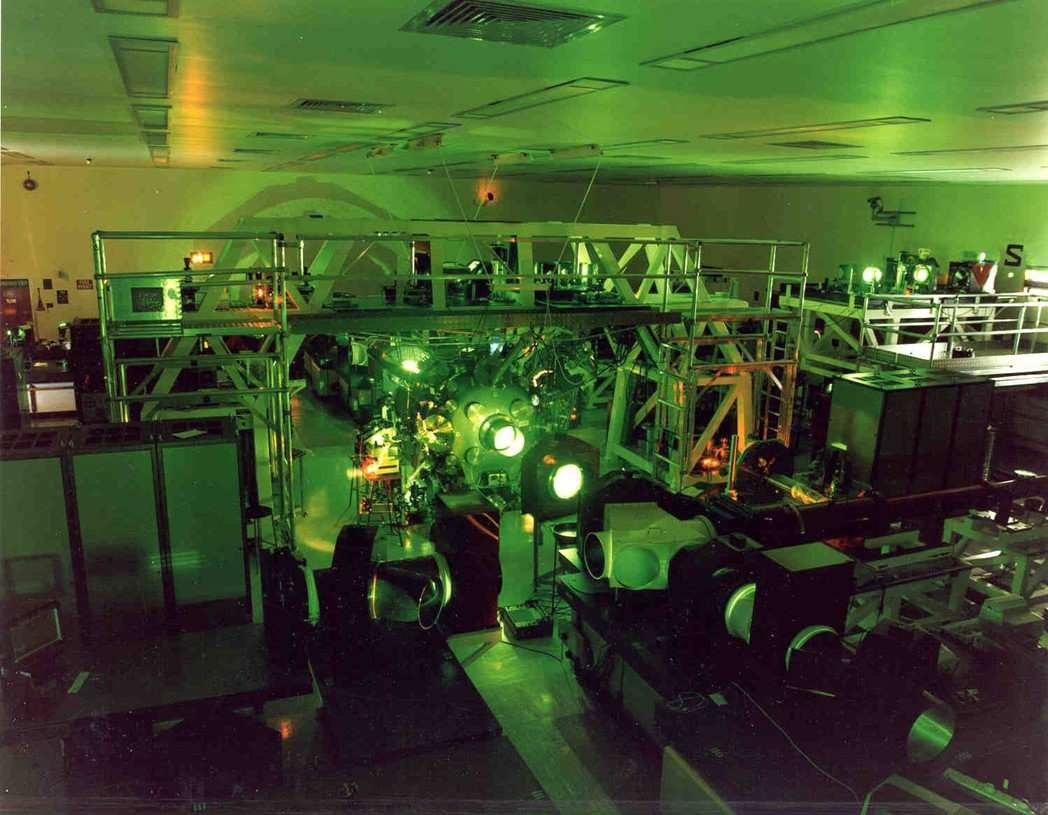
\includegraphics[width=0.78\textwidth]{../figures/as_helen_target.jpg}
\caption{英国 HELEN 激光装置的靶区：一束激光经过放大、转向与聚焦，最后打在一个毫米级靶点上。本节的高斯波束与准光学，讲的就是这一路上束宽怎么变。}
\label{fig:photo-appas3}
\figsource{Colin N. Danson 等，CC BY 4.0（Wikimedia Commons）}
\end{figure}

\section{高斯波束与准光学：把波当成有粗细的束}
\label{sec:app-as-beam}

射线没有粗细，真实的波束有。毫米波段的波束用高斯波束描述最方便：腰斑 $w_0$ 处最细，
往外按

\begin{equation}
w(z)=w_0\sqrt{1+\left(\frac{z}{z_R}\right)^2},
\qquad z_R=\frac{\pi w_0^2}{\lambda_0}
\label{eq:app-as-beam}
\end{equation}

张开。取发射腰斑 $w_0=2.0$ cm，则瑞利长度 $z_R=0.586837$ m，远场发散角

\begin{equation}
\theta_\mathrm{div}=\frac{\lambda_0}{\pi w_0}=0.0340810\ \mathrm{rad}=1.9527^\circ .
\label{eq:app-as-rayleigh}
\end{equation}

从边缘 $r=a$ 打到中心 $r=0$ 是 $2.0$ m：那里波束半径已经长到 $w=0.0710357$ m
（$z=1$ m 处 $0.0395160$ m，双程 $z=4$ m 处 $0.137783$ m，波前曲率半径 $R=2.17219$ m）。
腰斑处峰值强度 $2P/(\pi w_0^2)$ 对 $P=1.0$ MW 是 $1.59155\times10^{9}$ W m$^{-2}$，
到中心降到 $1.26162\times10^{8}$ W m$^{-2}$。

准光学要的是把功率压小。用焦距 $f=1.0$ m、口径 $D=0.20$ m 的镜面聚焦，焦斑腰斑

\begin{equation}
w_\mathrm{f}=\frac{\lambda_0 f}{\pi (D/2)}=0.00681621\ \mathrm{m}=6.81621\ \mathrm{mm},
\label{eq:app-as-focus}
\end{equation}

焦斑面积 $\pi w_\mathrm{f}^2=1.45961\times10^{-4}$ m$^2=145.961$ mm$^2$，峰值强度
$1.37023\times10^{10}$ W m$^{-2}$。强度换成电场用 $I=\tfrac12 c\epsilon_0 E^2$：

\begin{equation}
E_\mathrm{f}=\sqrt{\frac{2I_\mathrm{f}}{c\epsilon_0}}=3.21312\times10^{6}\ \mathrm{V\,m^{-1}}
=3.21312\ \mathrm{MV\,m^{-1}},
\label{eq:app-as-intensity}
\end{equation}

而等离子体中心处只有 $308.314$ kV m$^{-1}$。同一个 1 MW 波束，聚焦前后场强差了十倍——
这就是准光学设计存在的理由。

\begin{table}[htbp]
\centering
\small
\caption{1 MW、140 GHz 波束从发射到焦斑的几个尺寸}
\label{tab:app-as-beam}
\begin{tabular}{p{3.3cm}p{3.1cm}p{3.1cm}p{3.5cm}}
\hline
量 & 数值 & 位置 & 说明 \\
\hline
腰斑 $w_0$ & $2.0$ cm & 发射口 & 声明值 \\
瑞利长度 $z_R$ & $0.586837$ m & --- & 束宽涨到 $\sqrt2$ 倍 \\
发散角 $\theta_\mathrm{div}$ & $1.9527^\circ$ & 远场 & $0.0340810$ rad \\
束宽 $w$ & $0.0710357$ m & $z=2.0$ m & 打到中心 \\
峰值强度 & $1.59155\times10^{9}$ W m$^{-2}$ & 腰斑 & $2P/(\pi w_0^2)$ \\
峰值强度 & $1.26162\times10^{8}$ W m$^{-2}$ & 中心 & 散开之后 \\
焦斑 $w_\mathrm{f}$ & $6.81621$ mm & 镜后 & $f=1.0$ m、$D=0.20$ m \\
焦斑电场 $E_\mathrm{f}$ & $3.21312$ MV m$^{-1}$ & 焦斑 & 中心的 $10.42$ 倍 \\
\hline
\end{tabular}
\end{table}

\begin{tip}{准光学是把波长当成尺子}{tip-app-as-beam}
毫米波的器件尺寸和波长同量级：$140$ GHz 的波长 $2.14137$ mm，所以「镜面粗糙度、
腰斑、焦斑、间隙」都写作波长的倍数，而不是写作「几毫米」。做准光学设计时先把
$w_0/\lambda_0$ 算出来，再谈机械公差，顺序反了会白干。
\end{tip}

{\footnotesize
\textbf{出处：}高斯波束与聚焦腰斑的公式见 Born \& Wolf, \emph{Principles of Optics}
（第 7 版，1999）第 8 章与 Goldsmith, \emph{Quasioptical Systems}（1998）。
聚变装置上的准光学注入设计见 Thumm \& Kasparek, \emph{Fusion Engineering and Design}
（2002）。本附录不复制原书图。
}


\begin{figure}[htbp]
\centering
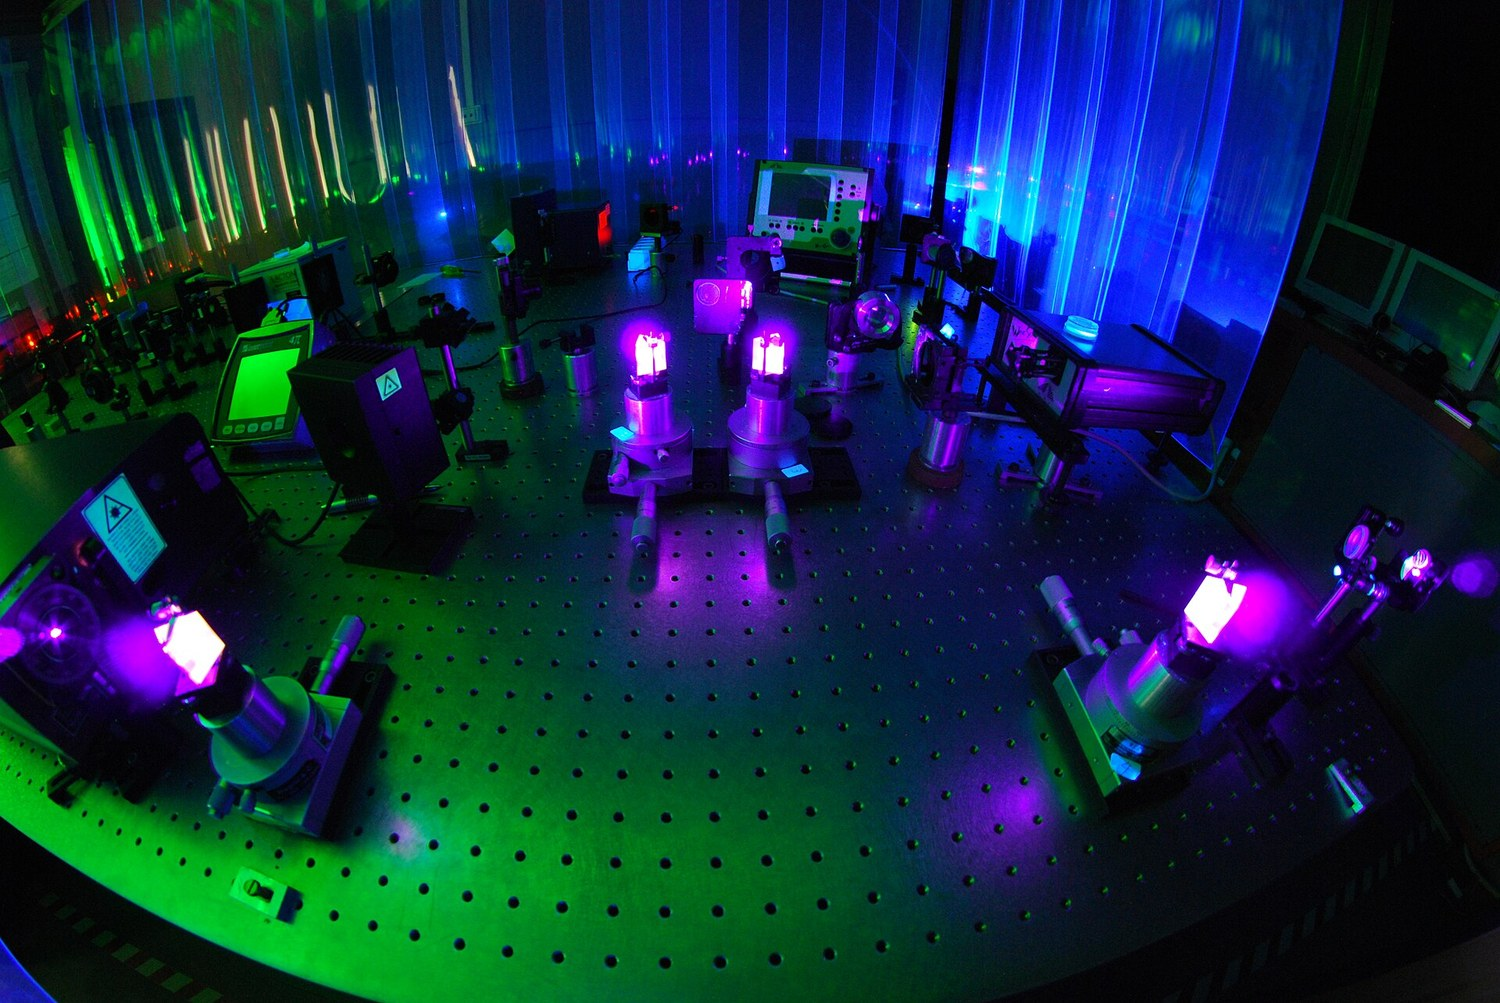
\includegraphics[width=0.72\textwidth]{../figures/optics_lab_inrim.jpg}
\caption{光学台：射线方程在这里被验证。把波长缩到远小于装置尺度时，波的传播就退化成本节的射线与准光学；光学台上那些反射镜与透镜，正是同一套射线方程在可见光波段的日常应用——微波诊断里的聚焦镜与它们遵循的是同一组公式。}
\label{fig:photo-appas}
\figsource{Giorgio Brida from Torino, Italy，CC BY 2.0（Wikimedia Commons）}
\end{figure}

\section{反射计：反射量的是时间，不是位置}
\label{sec:app-as-reflect}

反射计把一束毫米波垂直打进等离子体（O 模），波在 $n_\mathrm{e}=n_\mathrm{c}$ 的截止面上
折返，回来时测相位。相位随频率的变化率就是群延迟：

\begin{equation}
\phi(f)=\frac{4\pi f}{c}\int_{r_\mathrm{t}}^{a} n(r)\,\mathrm{d}r,
\qquad
\tau_\mathrm{g}(f)=\frac{1}{2\pi}\frac{\mathrm{d}\phi}{\mathrm{d}f}
=\frac{2}{c}\int_{r_\mathrm{t}}^{a}\frac{\mathrm{d}r}{n(r)} .
\label{eq:app-as-tau}
\end{equation}

O 模的 $n=\sqrt{1-n_\mathrm{e}/n_\mathrm{c}}$，所以频率扫到哪里，转折半径就落在哪个密度上：

\begin{equation}
r_\mathrm{t}(f)=a\sqrt{1-\frac{n_\mathrm{c}(f)}{n_\mathrm{e0}}},
\qquad n_\mathrm{c}(f)=1.24044\times10^{18}\left(\frac{f}{10\ \mathrm{GHz}}\right)^{2}
\ \mathrm{m^{-3}} .
\label{eq:app-as-profile}
\end{equation}

扫频从 $50$ GHz 到 $75$ GHz，转折半径从 $1.66119$ m（$0.830596a$）走到 $1.09955$ m
（$0.549774a$），覆盖了半个小半径。往返群延迟分别是 $4.66510$ ns、$7.19549$ ns 与
$13.4255$ ns；从 $50$ 到 $75$ GHz，半径跨过 $0.561644$ m，群延迟跨过 $8.76042$ ns，
平均灵敏度 $0.0224658$ m/GHz。

这个灵敏度决定了分辨率。相位分辨 $0.01$ rad 时，$75$ GHz 处的群延迟把频率分辨限在

\begin{equation}
\delta f=\frac{\delta\phi}{2\pi\tau_\mathrm{g}}=118.547\ \mathrm{kHz},
\qquad
\delta r=\left|\frac{\mathrm{d}r}{\mathrm{d}f}\right|\delta f=2.66324\ \mu\mathrm{m},
\label{eq:app-as-res}
\end{equation}

折合密度分辨 $1.46418\times10^{14}$ m$^{-3}$（相对 $2.09843\times10^{-6}$）。这是相位测量
本身的极限；真实系统里会先被密度剖面的模型误差吃掉。

同一个波束还可以测湍流的速度。斜着打、接收散射回来的波，多普勒频移给出垂直速度：

\begin{equation}
f_\mathrm{D}=\frac{2v_\perp\sin\theta_\mathrm{D}}{\lambda_0}
=3.19440\ \mathrm{MHz}
\qquad (v_\perp=1.0\times10^{4}\ \mathrm{m\,s^{-1}},\ \theta_\mathrm{D}=20^\circ),
\label{eq:app-as-doppler}
\end{equation}

多普勒谱的频率分辨 $100$ kHz 折合速度分辨 $313.048$ m s$^{-1}$。

\begin{table}[htbp]
\centering
\small
\caption{扫频反射计的三个通道：转折半径与往返时间}
\label{tab:app-as-reflect}
\begin{tabular}{p{2.2cm}p{2.9cm}p{2.6cm}p{2.6cm}p{2.5cm}}
\hline
频率 & 截止密度 & 转折半径 & 往返群延迟 & 相对半径 \\
\hline
$50$ GHz & $3.10111\times10^{19}$ m$^{-3}$ & $1.66119$ m & $4.66510$ ns & $0.830596a$ \\
$60$ GHz & $4.46559\times10^{19}$ m$^{-3}$ & $1.48787$ m & $7.19549$ ns & $0.743936a$ \\
$75$ GHz & $6.97749\times10^{19}$ m$^{-3}$ & $1.09955$ m & $13.4255$ ns & $0.549774a$ \\
\hline
\end{tabular}
\end{table}

\begin{tip}{反射计量的是时间，不是位置}{tip-app-as-reflect}
把「反射计测密度剖面」读成「反射计测位置」是最常见的误解：它测的是往返的相位与群延迟，
位置是靠模型反解出来的。所以剖面的正确性依赖两件事——折射率模型（O 模还是 X 模、
相对论修正）与转折几何（斜入射还是垂直入射）。
\end{tip}

{\footnotesize
\textbf{出处：}微波反射计的原理、群延迟与剖面反演见 Hutchinson, \emph{Principles of
Plasma Diagnostics}（第 2 版，2002）第 5 章与 Hartfuss \& Geist, \emph{Plasma Physics
and Controlled Fusion}（1998）。
多普勒反射计用于湍流速度测量见 Conway 等,
\emph{Plasma Physics and Controlled Fusion}（2004）。本附录不复制原书图表。
}


\section{电子回旋发射成像：共振面就是成像面}
\label{sec:app-as-ece}

电子在磁场里做回旋运动，就会辐射。回旋频率只由磁场决定：

\begin{equation}
f_\mathrm{ce}(r)=\frac{eB(r)}{2\pi m_\mathrm{e}}=2.79925\times10^{10}\,B\ \mathrm{Hz},
\qquad
B(r)=\frac{B_0R_0}{R_0+r},
\label{eq:app-as-ecefreq}
\end{equation}

所以「频率」和「半径」之间有确定的一一对应。轴上 $f_\mathrm{ce}=148.360$ GHz，二次谐波
$296.720$ GHz；到 $r=1.0$ m 降到 $127.755$ GHz（二次谐波 $255.509$ GHz），到边缘
$r=2.0$ m 是 $112.175$ GHz（$224.350$ GHz）。反过来，收到 $280$ GHz 的二次谐波辐射，
就知道它来自

\begin{equation}
r=\frac{B_0R_0}{B}-R_0=0.370237\ \mathrm{m},
\qquad
B=\frac{2\pi m_\mathrm{e}f_\mathrm{ce}}{e}=5.00134\ \mathrm{T}.
\label{eq:app-as-mapping}
\end{equation}

空间分辨由带宽定：在 $280$ GHz 处 $|\mathrm{d}r/\mathrm{d}f|=2.34651\times10^{-11}$ m/Hz，
$1$ GHz 带宽折合 $0.0234651$ m $=2.34651$ cm——比大多数湍流相关长度大，这就是为什么
ECE 成像要靠多通道阵列而不是单通道扫频。

辐射强度本身是热辐射。光学厚时亮度温度等于电子温度，瑞利--金斯极限给出

\begin{equation}
B_\nu=\frac{2\nu^2 k_\mathrm{B}T_\mathrm{e}}{c^2}
=2.56992\times10^{-9}\ \mathrm{W\,m^{-2}\,Hz^{-1}\,sr^{-1}}
\qquad (280\ \mathrm{GHz},\ T_\mathrm{e}=9.194\ \mathrm{keV}),
\label{eq:app-as-rj}
\end{equation}

单模接收（$A\Omega=\lambda^2$）在 $1$ GHz 带宽里拿到

\begin{equation}
P=B_\nu\,\delta f\,\lambda^2=2.94608\ \mu\mathrm{W},
\label{eq:app-as-ecepow}
\end{equation}

其中 $\lambda=1.07131$ mm。这个功率不大，但比任何自发的非热辐射都强得多——ECE 之所以
好用，就是因为它测的是「电子的体温」。

\begin{table}[htbp]
\centering
\small
\caption{二次谐波 ECE 的频率--半径对应（$B_0=5.3$ T，$R_0=6.2$ m）}
\label{tab:app-as-ece}
\begin{tabular}{p{2.5cm}p{2.4cm}p{2.6cm}p{2.6cm}p{2.7cm}}
\hline
半径 & 磁场 & $f_\mathrm{ce}$ & 二次谐波 & 说明 \\
\hline
$0$ m & $5.30000$ T & $148.360$ GHz & $296.720$ GHz & 轴上最高 \\
$0.370237$ m & $5.00134$ T & $140.000$ GHz & $280.000$ GHz & 本文算例通道 \\
$1.0$ m & $4.56389$ T & $127.755$ GHz & $255.509$ GHz & --- \\
$2.0$ m & $4.00732$ T & $112.175$ GHz & $224.350$ GHz & 边缘最低 \\
\hline
\end{tabular}
\end{table}

\begin{tip}{ECE 看到的是共振面，不是等离子体}{tip-app-as-ece}
ECE 的空间定位来自磁场，不来自光学：改变 $B_0$ 会把整个成像面平移。所以用 ECE 比较
不同放电的剖面之前，先把 $B_0$ 与 $R_0$ 对齐；否则看到的「温度变化」可能只是「位置
变化」。
\end{tip}

{\footnotesize
\textbf{出处：}电子回旋发射的诊断原理与光学厚度讨论见 Hutchinson（2002）第 6 章与
Mazzucato, \emph{Physics of Plasmas}（1998）。
成像 ECE 的通道设计见 Park 等,
\emph{Review of Scientific Instruments}（2006）。本附录不复制原书图表。
}


\section{功率沉积定位：共振面、多普勒展宽与沉积体积}
\label{sec:app-as-deposition}

加热用的波束最终要回答一个问题：功率落在哪里。冷共振条件 $f=f_\mathrm{ce}(r)$ 给出一个
面，但电子在动，真正的共振条件要把多普勒项算进去：

\begin{equation}
\omega-k_\parallel v_\parallel=\frac{\omega_\mathrm{ce}}{\gamma}
\approx\omega_\mathrm{ce},
\qquad k_\parallel=n_\parallel\frac{\omega}{c}.
\label{eq:app-as-resonance}
\end{equation}

本轮 $140$ GHz、$20^\circ$ 入射：$n_\parallel=n_\mathrm{p}\cos20^\circ=0.720991$，
热速度（一维多普勒宽度定义）$v_\parallel^\mathrm{th}=\sqrt{2k_\mathrm{B}T_\mathrm{e}/m_\mathrm{e}}=5.68693\times10^{7}$ m s$^{-1}$，
于是展宽量

\begin{equation}
\frac{\Delta\omega}{\omega}=n_\parallel\frac{v_\parallel^\mathrm{th}}{c}=0.136769 .
\label{eq:app-as-dopplerres}
\end{equation}

冷共振落在 $r=0.370237$ m；把 $+v_\parallel^\mathrm{th}$ 支代进去，共振面推到 $1.41121$ m
（外移 $1.04098$ m），$1/e$ 半宽就是 $1.04098$ m，整个展宽层厚 $2.08195$ m——比器壁到
中心的距离还大。$140$ GHz 在这个磁场里离轴上回旋频率（$148.36$ GHz）太近，是「共振面
贴着中心」的布置；若想沉积到更外面，要么降低 $B_0$，要么改用更高的谐波。

吸收功率本身由光学厚度定。取基频 O 模单程吸收份额 $\eta_\mathrm{abs}=0.95$（声明值），
则

\begin{equation}
P_\mathrm{abs}=\eta_\mathrm{abs}P_\mathrm{EC}=0.95\ \mathrm{MW},
\qquad
1-(1-\eta_\mathrm{abs})^2=0.9975\ \text{（双程）}.
\label{eq:app-as-abs}
\end{equation}

共振处波束半径 $w=0.0590350$ m，截面 $0.0109489$ m$^2$；把它摊到 $1/e$ 半宽上，平均
功率密度

\begin{equation}
\frac{P_\mathrm{abs}}{A_\mathrm{beam}\,\Delta r}
=\frac{9.5\times10^{5}}{0.0109489\times1.04098}
=5.48818\times10^{7}\ \mathrm{W\,m^{-3}} .
\label{eq:app-as-powerdens}
\end{equation}

作为对照：如果把同样的功率压进一个焦斑体积（$A_\mathrm{beam}\times2w_\mathrm{f}$），
密度会到 $6.36475\times10^{9}$ W m$^{-3}$，比实际的沉积密度高两个数量级。这正是
「射线告诉你落在哪，波束光学告诉你压得多紧」的分工。

\begin{table}[htbp]
\centering
\small
\caption{1 MW、140 GHz、$20^\circ$ 入射的沉积账}
\label{tab:app-as-deposition}
\begin{tabular}{p{3.4cm}p{3.1cm}p{3.0cm}p{3.5cm}}
\hline
量 & 数值 & 单位 & 说明 \\
\hline
冷共振半径 & $0.370237$ & m & $f=f_\mathrm{ce}$ \\
平行折射率 $n_\parallel$ & $0.720991$ & --- & $n_\mathrm{p}\cos20^\circ$ \\
多普勒展宽 $\Delta\omega/\omega$ & $0.136769$ & --- & $n_\parallel v_\parallel^\mathrm{th}/c$ \\
$+$ 支共振半径 & $1.41121$ & m & 外移 $1.04098$ m \\
展宽层厚 & $2.08195$ & m & 与器壁距离同量级 \\
吸收功率 $P_\mathrm{abs}$ & $0.95$ & MW & 单程 $95\%$（声明） \\
平均功率密度 & $5.48818\times10^{7}$ & W m$^{-3}$ & 摊在展宽层里 \\
焦斑极限密度 & $6.36475\times10^{9}$ & W m$^{-3}$ & 高两个数量级 \\
\hline
\end{tabular}
\end{table}

\begin{tip}{沉积位置由磁场和角度共同决定}{tip-app-as-deposition}
把「共振面」当成一个固定的环，是设计加热方案时最容易犯的错：同一个频率，入射角不同，
沉积半径可以差一米。多普勒展宽在 $140$ GHz 这种「低频、大角度」的布置下是主导项，
不是修正项。
\end{tip}

{\footnotesize
\textbf{出处：}电子回旋波的多普勒共振与功率沉积见 Bornatici 等, \emph{Nuclear Fusion}
（1983）与 ITER Physics Basis, \emph{Nuclear Fusion}（1999）第 6 章。
波束在等离子体
中的传播与吸收的数值方法见 Westerhof, \emph{Plasma Physics and Controlled Fusion}
（2000）。本附录不复制原书图表。
}


\section{估算练习}
\label{sec:app-as-problems}

\textbf{练习 1}
一束 $100$ GHz 的 O 模波垂直穿过密度 $n_\mathrm{e}=5.0\times10^{19}$ m$^{-3}$ 的等离子体。
求截止密度、折射率、波数，以及相速度是光速的多少倍。

\textbf{解答 1}
截止密度 $n_\mathrm{c}=1.24044\times10^{20}$ m$^{-3}$，$X=0.403082$，
$n=\sqrt{1-X}=0.772605$，波数
$k=2\pi f n/c=1619.26$ m$^{-1}$，相速度 $v_\mathrm{p}=c/n=3.88028\times10^{8}$ m s$^{-1}$，
即 $1.29432\,c$。相速度超过光速并不违反因果律：信息由群速度带走，而这里群速度
$v_\mathrm{g}=cn=0.772605\,c$，仍然小于光速。

\textbf{练习 2}
把发射腰斑从 $2.0$ cm 缩到 $1.0$ cm，瑞利长度与远场发散角各变成多少？

\textbf{解答 2}
$z_R=\pi w_0^2/\lambda_0$ 与 $w_0^2$ 成正比：腰斑减半，瑞利长度变成 $0.146709$ m
（原来的四分之一，原值 $0.586837$ m）；发散角 $\lambda_0/(\pi w_0)$ 与 $w_0$ 成反比，
变成 $3.90540^\circ$，正好是原来的两倍（原值 $1.9527^\circ$）。波束越细，散得越快。

\textbf{练习 3}
用 $70$ GHz 的反射计测密度剖面，转折半径落在哪里？往返群延迟是多少？

\textbf{解答 3}
$n_\mathrm{c}=6.07817\times10^{19}$ m$^{-3}$，转折半径
$r_\mathrm{t}=a\sqrt{1-n_\mathrm{c}/n_\mathrm{e0}}=1.25249$ m $=0.626245a$；
往返群延迟 $\tau_\mathrm{g}=(2/c)\int_{r_\mathrm{t}}^{a}\mathrm{d}r/n(r)
=1.08566\times10^{-8}$ s $=10.8566$ ns。作为对照，$60$ GHz 的转折半径是 $1.48787$ m、
群延迟 $7.19549$ ns，$75$ GHz 是 $1.09955$ m、$13.4255$ ns。

\textbf{练习 4}
多普勒反射计测到 $5.0$ MHz 的频移（$\lambda_0=2.14137$ mm、$\theta_\mathrm{D}=20^\circ$），
垂直速度是多少？

\textbf{解答 4}
$v_\perp=\lambda_0f_\mathrm{D}/(2\sin\theta_\mathrm{D})
=2.14137\times10^{-3}\times5.0\times10^{6}/(2\times0.342020)
=1.56524\times10^{4}$ m s$^{-1}$，即 $15.6524$ km s$^{-1}$。要测更慢的湍流，要么用更长的
波长，要么用更大的夹角。

\textbf{练习 5}
把 ECE 通道移到 $260$ GHz（二次谐波），它测的是哪个半径？$1$ GHz 带宽对应多厚的壳层？

\textbf{解答 5}
$B=2\pi m_\mathrm{e}f_\mathrm{ce}/e=4.64410$ T，$r=B_0R_0/B-R_0=0.875640$ m；
$|\mathrm{d}r/\mathrm{d}f|=2\,(\mathrm{d}B/\mathrm{d}f)$ 型换算给出
$1$ GHz 对应 $0.0272140$ m $=2.72140$ cm。比 $280$ GHz 通道的 $2.34651$ cm 稍厚——
越靠外，同样的带宽覆盖越厚。

\textbf{练习 6}
$2$ MW 的波束聚焦到 $w_\mathrm{f}=5$ mm，焦斑的峰值强度与电场是多少？与
$1$ MW、$w_\mathrm{f}=6.81621$ mm 的情形比呢？

\textbf{解答 6}
$I=2P/(\pi w_\mathrm{f}^2)=5.09296\times10^{10}$ W m$^{-2}$，
$E=\sqrt{2I/(c\epsilon_0)}=6.19463\times10^{6}$ V m$^{-1}=6.19463$ MV m$^{-1}$。
原来那组是 $1.37023\times10^{10}$ W m$^{-2}$ 与 $3.21312$ MV m$^{-1}$：功率翻倍、
焦斑面积缩到 $0.538089$ 倍，强度因此涨到 $3.71685$ 倍。

\section{来源、分级与版权说明}
\label{sec:app-as-source}

\begingroup\small
本附录的定位是「把波画成线、把线算成位置」：色散关系取自经典教材，射线方程与准光学
取自波动光学与聚变装置工程文献，诊断部分的通道参数按本书统一工作点复算。所有标出数值的
量都在 \texttt{tools/\allowbreak{}calc/\allowbreak{}appAS\_calc.py} 里重算过，没有从任何一本书的表格里搬数。

\begin{table}[htbp]
\centering
\small
\caption{本附录的借鉴来源与借用方式}
\label{tab:app-as-source}
\begin{tabular}{p{4.2cm}p{2.4cm}p{2.4cm}p{3.8cm}}
\hline
来源 & 用于 & 借用方式 & 版权说明 \\
\hline
Ginzburg 1964/1970 & AS.1--AS.2 & 色散关系与折射守恒 & 只复算，不复制图表 \\
Born \& Wolf 1999 & AS.3 & 高斯波束与聚焦公式 & 只复算，不复制图 \\
Goldsmith 1998 & AS.3 & 准光学量级判断 & 只借用方法 \\
Hutchinson 2002 & AS.4--AS.5 & 反射计与 ECE 原理 & 不复制公式表与图 \\
Tracy 等 2014 & AS.2 & 射线方程与波迹 & 只借用形式 \\
ITER Physics Basis 1999 & AS.6 & 多普勒共振与沉积 & 不复制剖面图 \\
\hline
\end{tabular}
\end{table}

\begin{tip}{本附录没有涵盖什么}{tip-app-as-honest}
本附录只在冷等离子体色散关系与线性几何光学里算路径、束宽与沉积位置。它不展开射线追踪
的具体数值算法（步长、插值、守恒量校验）、湍流对波束的散射、模式转换与隧穿的定量处理、
以及三维真实平衡下的波迹——这些要么在非线性与数值方法附录里，要么需要专门的波迹程序。
看到 $kL_n$ 掉到几十的量级，就该知道这一页的结论要打折。
\end{tip}

\textbf{出处：}本附录的「不复制」口径与全书一致：凡引用原书结论处只写结论与出处，
数值一律用 \texttt{tools/\allowbreak{}calc/\allowbreak{}appAS\_calc.py} 按 D1 工作点重算。射线追踪的工程实现可参考
Tracy 等（2014）与 Westerhof（2000）。
诊断通道参数与本书附录 Q 的同一组口径。
本附录不复制任何原书表格与图。
\endgroup